%!TeX root=../emmatop.tex
\chapter[Chapter \thechapter]{}
\lettrine[lraise=0.3]{A}{fter} being long fed with hopes of a speedy visit from Mr and Mrs Suckling, the Highbury world were obliged to endure the mortification of hearing that they could not possibly come till the autumn. No such importation of novelties could enrich their intellectual stores at present. In the daily interchange of news, they must be again restricted to the other topics with which for a while the Sucklings' coming had been united, such as the last accounts of Mrs Churchill, whose health seemed every day to supply a different report, and the situation of Mrs Weston, whose happiness it was to be hoped might eventually be as much increased by the arrival of a child, as that of all her neighbours was by the approach of it.

Mrs Elton was very much disappointed. It was the delay of a great deal of pleasure and parade. Her introductions and recommendations must all wait, and every projected party be still only talked of. So she thought at first;—but a little consideration convinced her that every thing need not be put off. Why should not they explore to Box Hill though the Sucklings did not come? They could go there again with them in the autumn. It was settled that they should go to Box Hill. That there was to be such a party had been long generally known: it had even given the idea of another. Emma had never been to Box Hill; she wished to see what every body found so well worth seeing, and she and Mr Weston had agreed to chuse some fine morning and drive thither. Two or three more of the chosen only were to be admitted to join them, and it was to be done in a quiet, unpretending, elegant way, infinitely superior to the bustle and preparation, the regular eating and drinking, and picnic parade of the Eltons and the Sucklings.

This was so very well understood between them, that Emma could not but feel some surprise, and a little displeasure, on hearing from Mr Weston that he had been proposing to Mrs Elton, as her brother and sister had failed her, that the two parties should unite, and go together; and that as Mrs Elton had very readily acceded to it, so it was to be, if she had no objection. Now, as her objection was nothing but her very great dislike of Mrs Elton, of which Mr Weston must already be perfectly aware, it was not worth bringing forward again:—it could not be done without a reproof to him, which would be giving pain to his wife; and she found herself therefore obliged to consent to an arrangement which she would have done a great deal to avoid; an arrangement which would probably expose her even to the degradation of being said to be of Mrs Elton's party! Every feeling was offended; and the forbearance of her outward submission left a heavy arrear due of secret severity in her reflections on the unmanageable goodwill of Mr Weston's temper.

<I am glad you approve of what I have done,> said he very comfortably. <But I thought you would. Such schemes as these are nothing without numbers. One cannot have too large a party. A large party secures its own amusement. And she is a good-natured woman after all. One could not leave her out.>

Emma denied none of it aloud, and agreed to none of it in private.

It was now the middle of June, and the weather fine; and Mrs Elton was growing impatient to name the day, and settle with Mr Weston as to pigeon-pies and cold lamb, when a lame carriage-horse threw every thing into sad uncertainty. It might be weeks, it might be only a few days, before the horse were useable; but no preparations could be ventured on, and it was all melancholy stagnation. Mrs Elton's resources were inadequate to such an attack.

<Is not this most vexatious, Knightley?> she cried.—<And such weather for exploring!—These delays and disappointments are quite odious. What are we to do?—The year will wear away at this rate, and nothing done. Before this time last year I assure you we had had a delightful exploring party from Maple Grove to Kings Weston.>

<You had better explore to Donwell,> replied Mr Knightley. <That may be done without horses. Come, and eat my strawberries. They are ripening fast.>

If Mr Knightley did not begin seriously, he was obliged to proceed so, for his proposal was caught at with delight; and the <Oh! I should like it of all things,> was not plainer in words than manner. Donwell was famous for its strawberry-beds, which seemed a plea for the invitation: but no plea was necessary; cabbage-beds would have been enough to tempt the lady, who only wanted to be going somewhere. She promised him again and again to come—much oftener than he doubted—and was extremely gratified by such a proof of intimacy, such a distinguishing compliment as she chose to consider it.

<You may depend upon me,> said she. <I certainly will come. Name your day, and I will come. You will allow me to bring Jane Fairfax?>

<I cannot name a day,> said he, <till I have spoken to some others whom I would wish to meet you.>

<Oh! leave all that to me. Only give me a carte-blanche.—I am Lady Patroness, you know. It is my party. I will bring friends with me.>

<I hope you will bring Elton,> said he: <but I will not trouble you to give any other invitations.>

\begin{figure}[tbph]
\centering
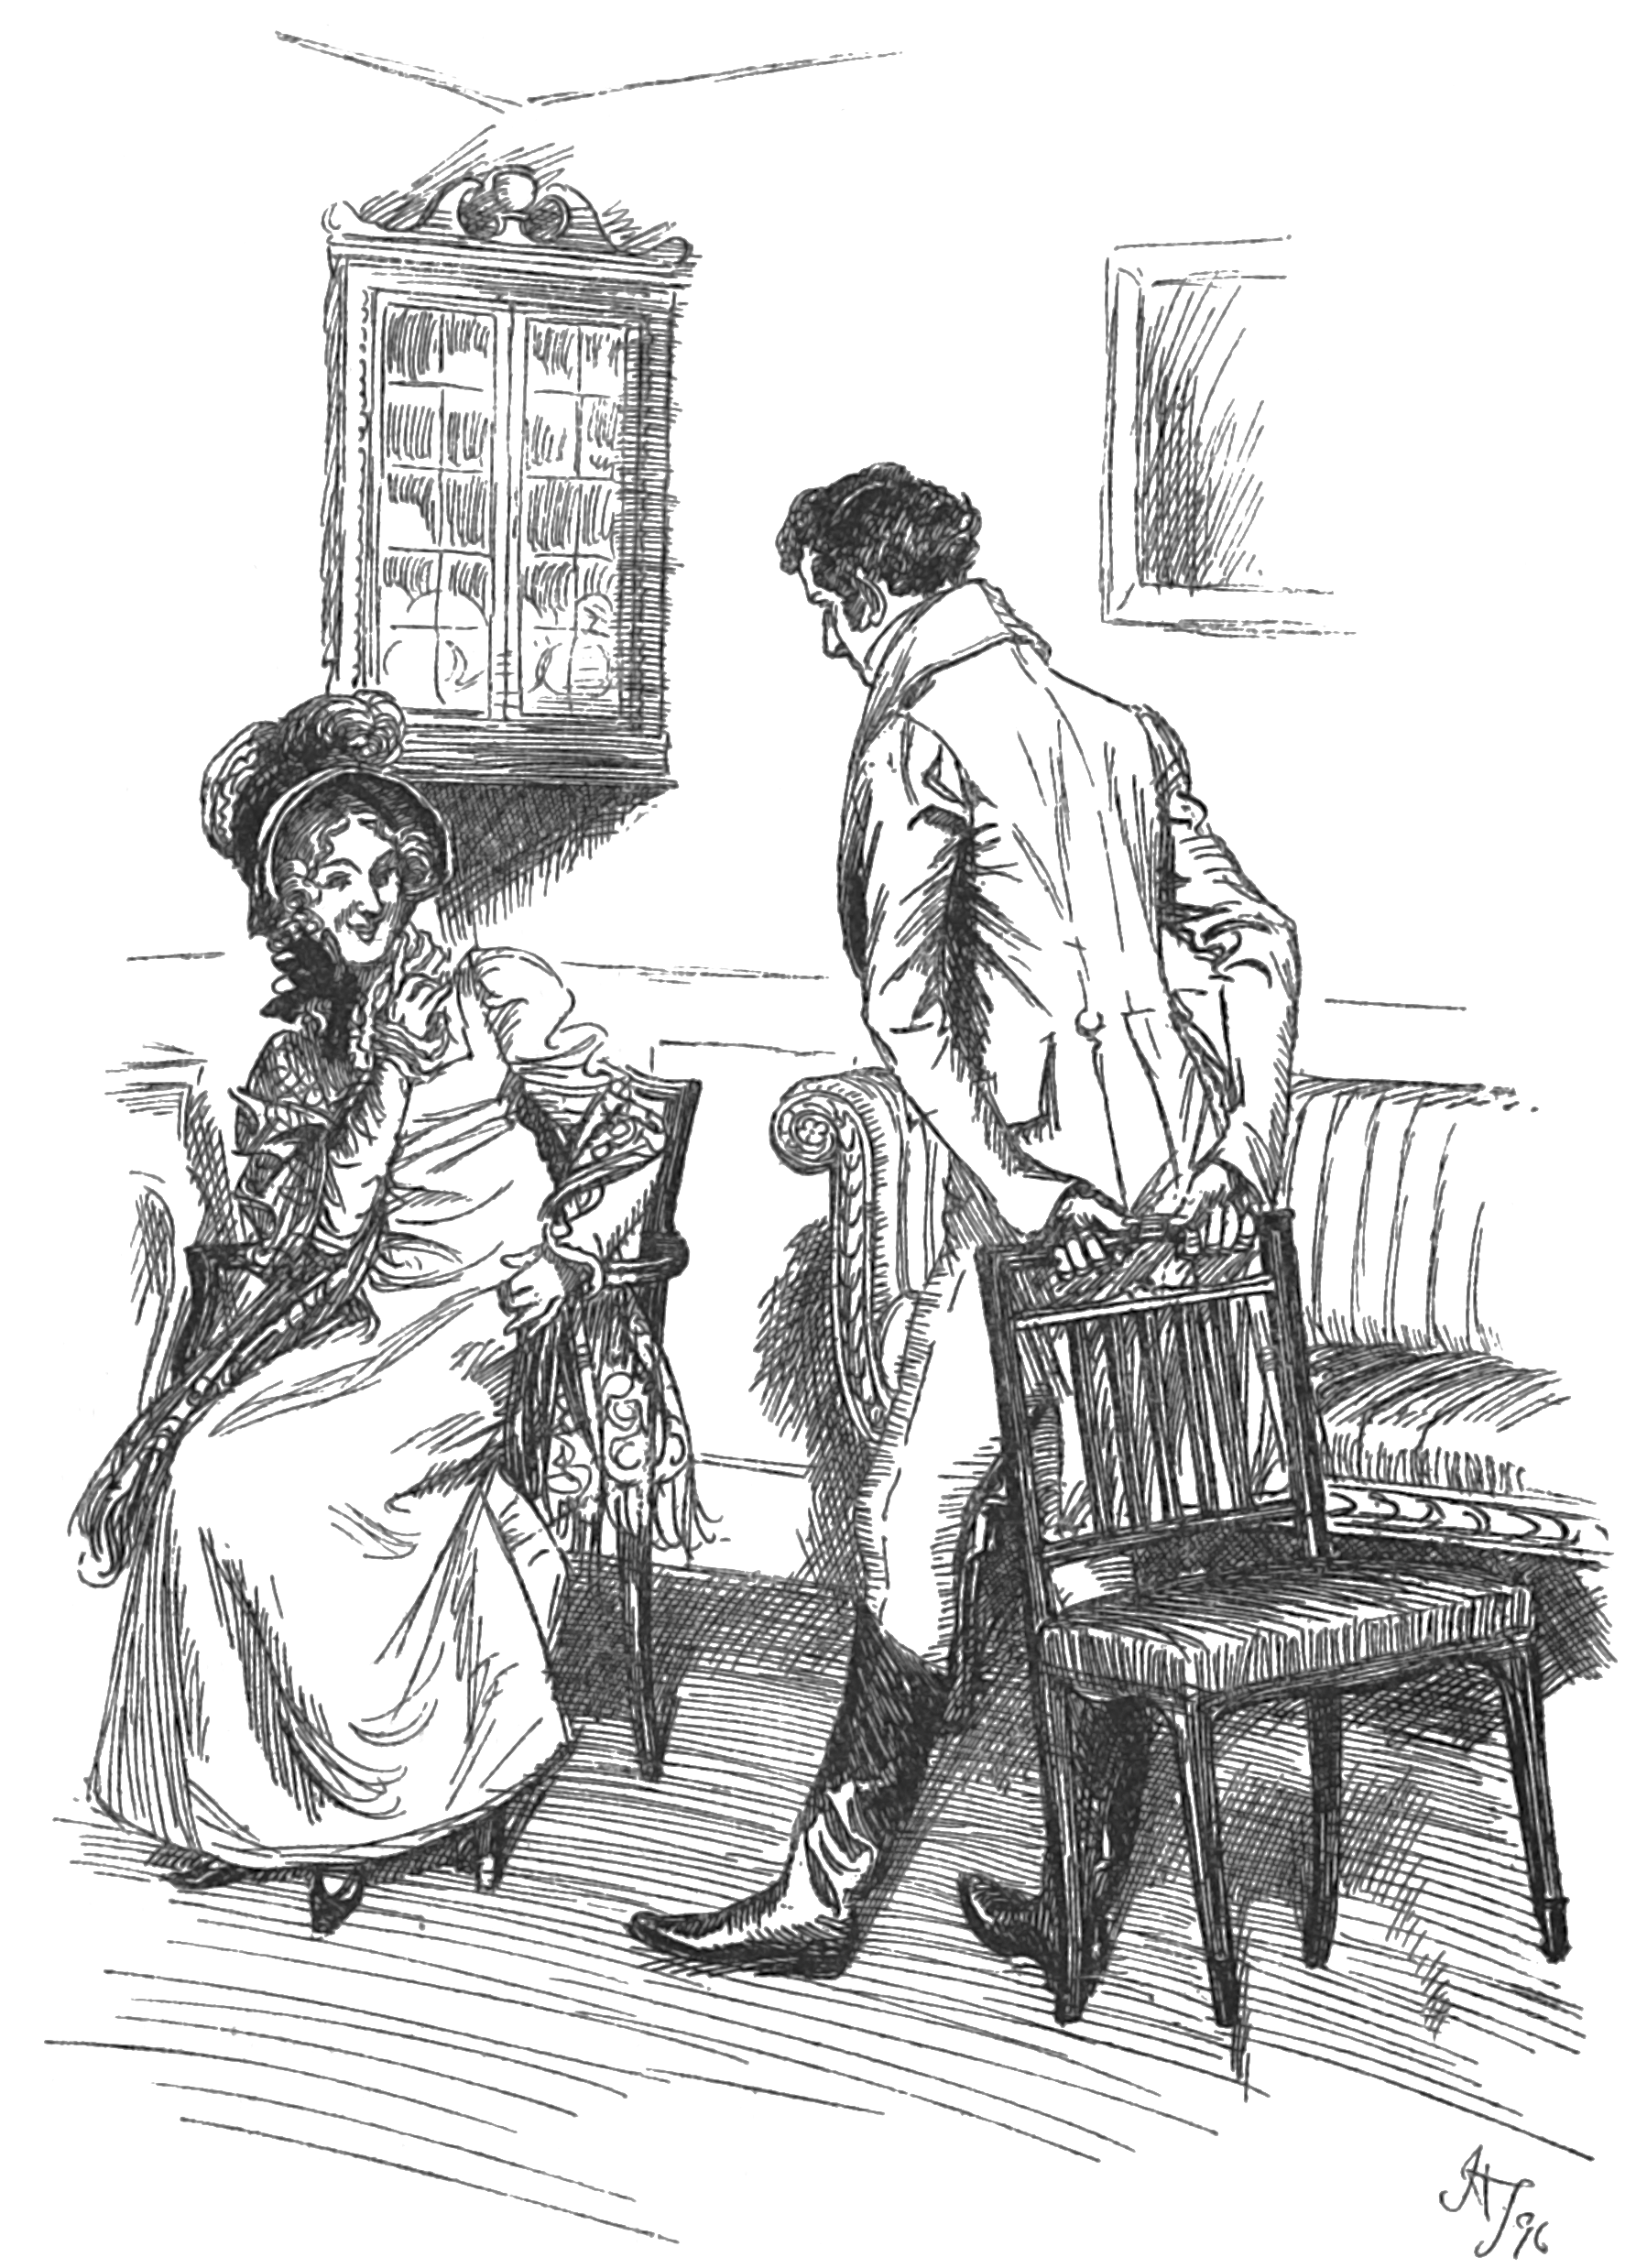
\includegraphics[width=\linewidth]{42sly}
\caption{<Oh! now you are looking very sly.>}
\end{figure}


<Oh! now you are looking very sly. But consider—you need not be afraid of delegating power to me. I am no young lady on her preferment. Married women, you know, may be safely authorised. It is my party. Leave it all to me. I will invite your guests.>

<No,>—he calmly replied,—<there is but one married woman in the world whom I can ever allow to invite what guests she pleases to Donwell, and that one is\longdash>

<—Mrs Weston, I suppose,> interrupted Mrs Elton, rather mortified.

<No—Mrs Knightley;—and till she is in being, I will manage such matters myself.>

<Ah! you are an odd creature!> she cried, satisfied to have no one preferred to herself.—<You are a humourist, and may say what you like. Quite a humourist. Well, I shall bring Jane with me—Jane and her aunt.—The rest I leave to you. I have no objections at all to meeting the Hartfield family. Don't scruple. I know you are attached to them.>

<You certainly will meet them if I can prevail; and I shall call on Miss Bates in my way home.>

<That's quite unnecessary; I see Jane every day:—but as you like. It is to be a morning scheme, you know, Knightley; quite a simple thing. I shall wear a large bonnet, and bring one of my little baskets hanging on my arm. Here,—probably this basket with pink ribbon. Nothing can be more simple, you see. And Jane will have such another. There is to be no form or parade—a sort of gipsy party. We are to walk about your gardens, and gather the strawberries ourselves, and sit under trees;—and whatever else you may like to provide, it is to be all out of doors—a table spread in the shade, you know. Every thing as natural and simple as possible. Is not that your idea?>

<Not quite. My idea of the simple and the natural will be to have the table spread in the dining-room. The nature and the simplicity of gentlemen and ladies, with their servants and furniture, I think is best observed by meals within doors. When you are tired of eating strawberries in the garden, there shall be cold meat in the house.>

<Well—as you please; only don't have a great set out. And, by the bye, can I or my housekeeper be of any use to you with our opinion?—Pray be sincere, Knightley. If you wish me to talk to Mrs Hodges, or to inspect anything\longdash>

<I have not the least wish for it, I thank you.>

<Well—but if any difficulties should arise, my housekeeper is extremely clever.>

<I will answer for it, that mine thinks herself full as clever, and would spurn any body's assistance.>

<I wish we had a donkey. The thing would be for us all to come on donkeys, Jane, Miss Bates, and me—and my caro sposo walking by. I really must talk to him about purchasing a donkey. In a country life I conceive it to be a sort of necessary; for, let a woman have ever so many resources, it is not possible for her to be always shut up at home;—and very long walks, you know—in summer there is dust, and in winter there is dirt.>

<You will not find either, between Donwell and Highbury. Donwell Lane is never dusty, and now it is perfectly dry. Come on a donkey, however, if you prefer it. You can borrow Mrs Cole's. I would wish every thing to be as much to your taste as possible.>

<That I am sure you would. Indeed I do you justice, my good friend. Under that peculiar sort of dry, blunt manner, I know you have the warmest heart. As I tell Mr E., you are a thorough humourist.—Yes, believe me, Knightley, I am fully sensible of your attention to me in the whole of this scheme. You have hit upon the very thing to please me.>

Mr Knightley had another reason for avoiding a table in the shade. He wished to persuade Mr Woodhouse, as well as Emma, to join the party; and he knew that to have any of them sitting down out of doors to eat would inevitably make him ill. Mr Woodhouse must not, under the specious pretence of a morning drive, and an hour or two spent at Donwell, be tempted away to his misery.

He was invited on good faith. No lurking horrors were to upbraid him for his easy credulity. He did consent. He had not been at Donwell for two years. <Some very fine morning, he, and Emma, and Harriet, could go very well; and he could sit still with Mrs Weston, while the dear girls walked about the gardens. He did not suppose they could be damp now, in the middle of the day. He should like to see the old house again exceedingly, and should be very happy to meet Mr and Mrs Elton, and any other of his neighbours.—He could not see any objection at all to his, and Emma's, and Harriet's going there some very fine morning. He thought it very well done of Mr Knightley to invite them—very kind and sensible—much cleverer than dining out.—He was not fond of dining out.>

Mr Knightley was fortunate in every body's most ready concurrence. The invitation was everywhere so well received, that it seemed as if, like Mrs Elton, they were all taking the scheme as a particular compliment to themselves.—Emma and Harriet professed very high expectations of pleasure from it; and Mr Weston, unasked, promised to get Frank over to join them, if possible; a proof of approbation and gratitude which could have been dispensed with.—Mr Knightley was then obliged to say that he should be glad to see him; and Mr Weston engaged to lose no time in writing, and spare no arguments to induce him to come.

In the meanwhile the lame horse recovered so fast, that the party to Box Hill was again under happy consideration; and at last Donwell was settled for one day, and Box Hill for the next,—the weather appearing exactly right.

Under a bright mid-day sun, at almost Midsummer, Mr Woodhouse was safely conveyed in his carriage, with one window down, to partake of this al-fresco party; and in one of the most comfortable rooms in the Abbey, especially prepared for him by a fire all the morning, he was happily placed, quite at his ease, ready to talk with pleasure of what had been achieved, and advise every body to come and sit down, and not to heat themselves.—Mrs Weston, who seemed to have walked there on purpose to be tired, and sit all the time with him, remained, when all the others were invited or persuaded out, his patient listener and sympathiser.

It was so long since Emma had been at the Abbey, that as soon as she was satisfied of her father's comfort, she was glad to leave him, and look around her; eager to refresh and correct her memory with more particular observation, more exact understanding of a house and grounds which must ever be so interesting to her and all her family.

She felt all the honest pride and complacency which her alliance with the present and future proprietor could fairly warrant, as she viewed the respectable size and style of the building, its suitable, becoming, characteristic situation, low and sheltered—its ample gardens stretching down to meadows washed by a stream, of which the Abbey, with all the old neglect of prospect, had scarcely a sight—and its abundance of timber in rows and avenues, which neither fashion nor extravagance had rooted up.—The house was larger than Hartfield, and totally unlike it, covering a good deal of ground, rambling and irregular, with many comfortable, and one or two handsome rooms.—It was just what it ought to be, and it looked what it was—and Emma felt an increasing respect for it, as the residence of a family of such true gentility, untainted in blood and understanding.—Some faults of temper John Knightley had; but Isabella had connected herself unexceptionably. She had given them neither men, nor names, nor places, that could raise a blush. These were pleasant feelings, and she walked about and indulged them till it was necessary to do as the others did, and collect round the strawberry-beds.—The whole party were assembled, excepting Frank Churchill, who was expected every moment from Richmond; and Mrs Elton, in all her apparatus of happiness, her large bonnet and her basket, was very ready to lead the way in gathering, accepting, or talking—strawberries, and only strawberries, could now be thought or spoken of.—<The best fruit in England—every body's favourite—always wholesome.—These the finest beds and finest sorts.—Delightful to gather for one's self—the only way of really enjoying them.—Morning decidedly the best time—never tired—every sort good—hautboy infinitely superior—no comparison—the others hardly eatable—hautboys very scarce—Chili preferred—white wood finest flavour of all—price of strawberries in London—abundance about Bristol—Maple Grove—cultivation—beds when to be renewed—gardeners thinking exactly different—no general rule—gardeners never to be put out of their way—delicious fruit—only too rich to be eaten much of—inferior to cherries—currants more refreshing—only objection to gathering strawberries the stooping—glaring sun—tired to death—could bear it no longer—must go and sit in the shade.>

Such, for half an hour, was the conversation—interrupted only once by Mrs Weston, who came out, in her solicitude after her son-in-law, to inquire if he were come—and she was a little uneasy.—She had some fears of his horse.

Seats tolerably in the shade were found; and now Emma was obliged to overhear what Mrs Elton and Jane Fairfax were talking of.—A situation, a most desirable situation, was in question. Mrs Elton had received notice of it that morning, and was in raptures. It was not with Mrs Suckling, it was not with Mrs Bragge, but in felicity and splendour it fell short only of them: it was with a cousin of Mrs Bragge, an acquaintance of Mrs Suckling, a lady known at Maple Grove. Delightful, charming, superior, first circles, spheres, lines, ranks, every thing—and Mrs Elton was wild to have the offer closed with immediately.—On her side, all was warmth, energy, and triumph—and she positively refused to take her friend's negative, though Miss Fairfax continued to assure her that she would not at present engage in any thing, repeating the same motives which she had been heard to urge before.—Still Mrs Elton insisted on being authorised to write an acquiescence by the morrow's post.—How Jane could bear it at all, was astonishing to Emma.—She did look vexed, she did speak pointedly—and at last, with a decision of action unusual to her, proposed a removal.—<Should not they walk? Would not Mr Knightley shew them the gardens—all the gardens?—She wished to see the whole extent.>—The pertinacity of her friend seemed more than she could bear.

It was hot; and after walking some time over the gardens in a scattered, dispersed way, scarcely any three together, they insensibly followed one another to the delicious shade of a broad short avenue of limes, which stretching beyond the garden at an equal distance from the river, seemed the finish of the pleasure grounds.—It led to nothing; nothing but a view at the end over a low stone wall with high pillars, which seemed intended, in their erection, to give the appearance of an approach to the house, which never had been there. Disputable, however, as might be the taste of such a termination, it was in itself a charming walk, and the view which closed it extremely pretty.—The considerable slope, at nearly the foot of which the Abbey stood, gradually acquired a steeper form beyond its grounds; and at half a mile distant was a bank of considerable abruptness and grandeur, well clothed with wood;—and at the bottom of this bank, favourably placed and sheltered, rose the Abbey Mill Farm, with meadows in front, and the river making a close and handsome curve around it.

It was a sweet view—sweet to the eye and the mind. English verdure, English culture, English comfort, seen under a sun bright, without being oppressive.

In this walk Emma and Mr Weston found all the others assembled; and towards this view she immediately perceived Mr Knightley and Harriet distinct from the rest, quietly leading the way. Mr Knightley and Harriet!—It was an odd tête-à-tête; but she was glad to see it.—There had been a time when he would have scorned her as a companion, and turned from her with little ceremony. Now they seemed in pleasant conversation. There had been a time also when Emma would have been sorry to see Harriet in a spot so favourable for the Abbey Mill Farm; but now she feared it not. It might be safely viewed with all its appendages of prosperity and beauty, its rich pastures, spreading flocks, orchard in blossom, and light column of smoke ascending.—She joined them at the wall, and found them more engaged in talking than in looking around. He was giving Harriet information as to modes of agriculture, etc. and Emma received a smile which seemed to say, <These are my own concerns. I have a right to talk on such subjects, without being suspected of introducing Robert Martin.>—She did not suspect him. It was too old a story.—Robert Martin had probably ceased to think of Harriet.—They took a few turns together along the walk.—The shade was most refreshing, and Emma found it the pleasantest part of the day.

The next remove was to the house; they must all go in and eat;—and they were all seated and busy, and still Frank Churchill did not come. Mrs Weston looked, and looked in vain. His father would not own himself uneasy, and laughed at her fears; but she could not be cured of wishing that he would part with his black mare. He had expressed himself as to coming, with more than common certainty. <His aunt was so much better, that he had not a doubt of getting over to them.>—Mrs Churchill's state, however, as many were ready to remind her, was liable to such sudden variation as might disappoint her nephew in the most reasonable dependence—and Mrs Weston was at last persuaded to believe, or to say, that it must be by some attack of Mrs Churchill that he was prevented coming.—Emma looked at Harriet while the point was under consideration; she behaved very well, and betrayed no emotion.

The cold repast was over, and the party were to go out once more to see what had not yet been seen, the old Abbey fish-ponds; perhaps get as far as the clover, which was to be begun cutting on the morrow, or, at any rate, have the pleasure of being hot, and growing cool again.—Mr Woodhouse, who had already taken his little round in the highest part of the gardens, where no damps from the river were imagined even by him, stirred no more; and his daughter resolved to remain with him, that Mrs Weston might be persuaded away by her husband to the exercise and variety which her spirits seemed to need.

Mr Knightley had done all in his power for Mr Woodhouse's entertainment. Books of engravings, drawers of medals, cameos, corals, shells, and every other family collection within his cabinets, had been prepared for his old friend, to while away the morning; and the kindness had perfectly answered. Mr Woodhouse had been exceedingly well amused. Mrs Weston had been shewing them all to him, and now he would shew them all to Emma;—fortunate in having no other resemblance to a child, than in a total want of taste for what he saw, for he was slow, constant, and methodical.—Before this second looking over was begun, however, Emma walked into the hall for the sake of a few moments' free observation of the entrance and ground-plot of the house—and was hardly there, when Jane Fairfax appeared, coming quickly in from the garden, and with a look of escape.—Little expecting to meet Miss Woodhouse so soon, there was a start at first; but Miss Woodhouse was the very person she was in quest of.

<Will you be so kind,> said she, <when I am missed, as to say that I am gone home?—I am going this moment.—My aunt is not aware how late it is, nor how long we have been absent—but I am sure we shall be wanted, and I am determined to go directly.—I have said nothing about it to any body. It would only be giving trouble and distress. Some are gone to the ponds, and some to the lime walk. Till they all come in I shall not be missed; and when they do, will you have the goodness to say that I am gone?>

<Certainly, if you wish it;—but you are not going to walk to Highbury alone?>

<Yes—what should hurt me?—I walk fast. I shall be at home in twenty minutes.>

<But it is too far, indeed it is, to be walking quite alone. Let my father's servant go with you.—Let me order the carriage. It can be round in five minutes.>

<Thank you, thank you—but on no account.—I would rather walk.—And for me to be afraid of walking alone!—I, who may so soon have to guard others!>

She spoke with great agitation; and Emma very feelingly replied, <That can be no reason for your being exposed to danger now. I must order the carriage. The heat even would be danger.—You are fatigued already.>

<I am,>—she answered—<I am fatigued; but it is not the sort of fatigue—quick walking will refresh me.—Miss Woodhouse, we all know at times what it is to be wearied in spirits. Mine, I confess, are exhausted. The greatest kindness you can shew me, will be to let me have my own way, and only say that I am gone when it is necessary.>

Emma had not another word to oppose. She saw it all; and entering into her feelings, promoted her quitting the house immediately, and watched her safely off with the zeal of a friend. Her parting look was grateful—and her parting words, <Oh! Miss Woodhouse, the comfort of being sometimes alone!>—seemed to burst from an overcharged heart, and to describe somewhat of the continual endurance to be practised by her, even towards some of those who loved her best.

<Such a home, indeed! such an aunt!> said Emma, as she turned back into the hall again. <I do pity you. And the more sensibility you betray of their just horrors, the more I shall like you.>

Jane had not been gone a quarter of an hour, and they had only accomplished some views of St Mark's Place, Venice, when Frank Churchill entered the room. Emma had not been thinking of him, she had forgotten to think of him—but she was very glad to see him. Mrs Weston would be at ease. The black mare was blameless; they were right who had named Mrs Churchill as the cause. He had been detained by a temporary increase of illness in her; a nervous seizure, which had lasted some hours—and he had quite given up every thought of coming, till very late;—and had he known how hot a ride he should have, and how late, with all his hurry, he must be, he believed he should not have come at all. The heat was excessive; he had never suffered any thing like it—almost wished he had staid at home—nothing killed him like heat—he could bear any degree of cold, etc., but heat was intolerable—and he sat down, at the greatest possible distance from the slight remains of Mr Woodhouse's fire, looking very deplorable.

<You will soon be cooler, if you sit still,> said Emma.

<As soon as I am cooler I shall go back again. I could very ill be spared—but such a point had been made of my coming! You will all be going soon I suppose; the whole party breaking up. I met one as I came—Madness in such weather!—absolute madness!>

Emma listened, and looked, and soon perceived that Frank Churchill's state might be best defined by the expressive phrase of being out of humour. Some people were always cross when they were hot. Such might be his constitution; and as she knew that eating and drinking were often the cure of such incidental complaints, she recommended his taking some refreshment; he would find abundance of every thing in the dining-room—and she humanely pointed out the door.

<No—he should not eat. He was not hungry; it would only make him hotter.> In two minutes, however, he relented in his own favour; and muttering something about spruce-beer, walked off. Emma returned all her attention to her father, saying in secret—

<I am glad I have done being in love with him. I should not like a man who is so soon discomposed by a hot morning. Harriet's sweet easy temper will not mind it.>

\begin{figure}[tbph]
\centering
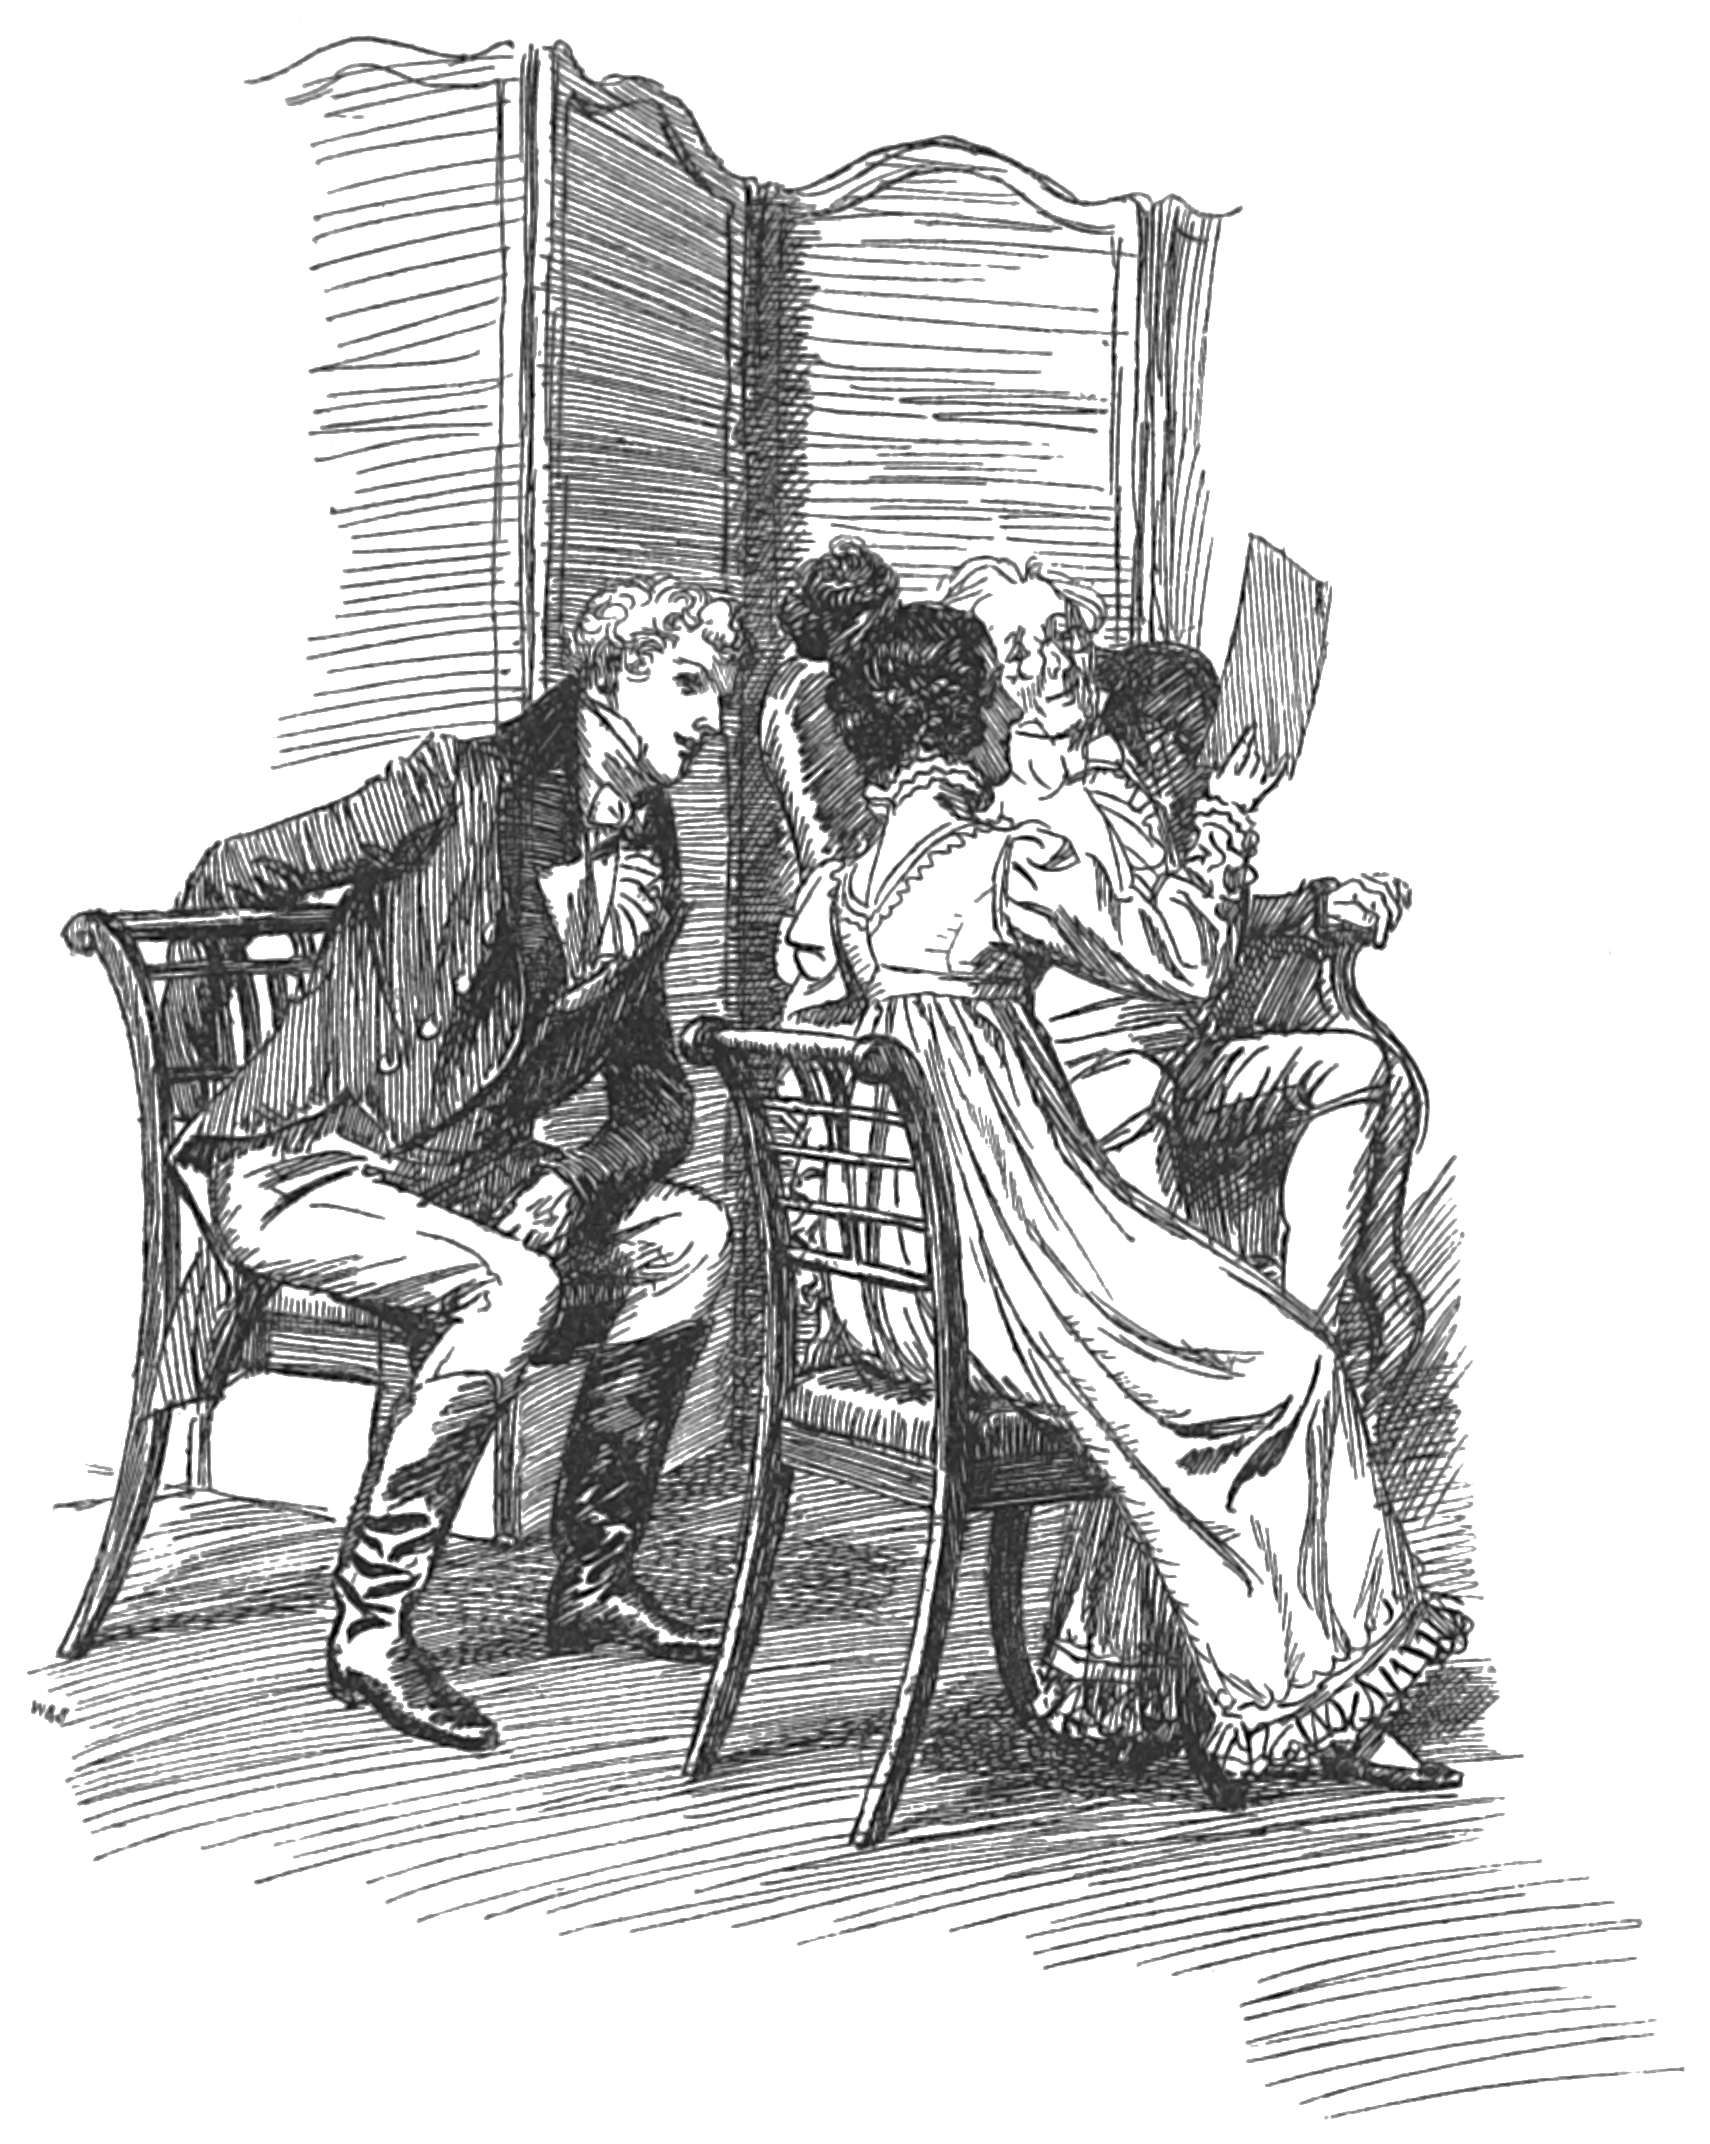
\includegraphics[width=\linewidth]{42employment}
\caption{Able to take an interest in their employment}
\end{figure}

He was gone long enough to have had a very comfortable meal, and came back all the better—grown quite cool—and, with good manners, like himself—able to draw a chair close to them, take an interest in their employment; and regret, in a reasonable way, that he should be so late. He was not in his best spirits, but seemed trying to improve them; and, at last, made himself talk nonsense very agreeably. They were looking over views in Swisserland.

<As soon as my aunt gets well, I shall go abroad,> said he. <I shall never be easy till I have seen some of these places. You will have my sketches, some time or other, to look at—or my tour to read—or my poem. I shall do something to expose myself.>

<That may be—but not by sketches in Swisserland. You will never go to Swisserland. Your uncle and aunt will never allow you to leave England.>

<They may be induced to go too. A warm climate may be prescribed for her. I have more than half an expectation of our all going abroad. I assure you I have. I feel a strong persuasion, this morning, that I shall soon be abroad. I ought to travel. I am tired of doing nothing. I want a change. I am serious, Miss Woodhouse, whatever your penetrating eyes may fancy—I am sick of England—and would leave it to-morrow, if I could.>

<You are sick of prosperity and indulgence. Cannot you invent a few hardships for yourself, and be contented to stay?>

<\textit{I} sick of prosperity and indulgence! You are quite mistaken. I do not look upon myself as either prosperous or indulged. I am thwarted in every thing material. I do not consider myself at all a fortunate person.>

<You are not quite so miserable, though, as when you first came. Go and eat and drink a little more, and you will do very well. Another slice of cold meat, another draught of Madeira and water, will make you nearly on a par with the rest of us.>

<No—I shall not stir. I shall sit by you. You are my best cure.>

<We are going to Box Hill to-morrow;—you will join us. It is not Swisserland, but it will be something for a young man so much in want of a change. You will stay, and go with us?>

<No, certainly not; I shall go home in the cool of the evening.>

<But you may come again in the cool of to-morrow morning.>

<No—It will not be worth while. If I come, I shall be cross.>

<Then pray stay at Richmond.>

<But if I do, I shall be crosser still. I can never bear to think of you all there without me.>

<These are difficulties which you must settle for yourself. Chuse your own degree of crossness. I shall press you no more.>

The rest of the party were now returning, and all were soon collected. With some there was great joy at the sight of Frank Churchill; others took it very composedly; but there was a very general distress and disturbance on Miss Fairfax's disappearance being explained. That it was time for every body to go, concluded the subject; and with a short final arrangement for the next day's scheme, they parted. Frank Churchill's little inclination to exclude himself increased so much, that his last words to Emma were,

<Well;—if you wish me to stay and join the party, I will.>

She smiled her acceptance; and nothing less than a summons from Richmond was to take him back before the following evening.